\documentclass{article}
\usepackage[T1]{fontenc}
\usepackage{amsmath}
\usepackage{listings}
\usepackage{xcolor}
\usepackage{graphicx}

\definecolor{codegreen}{rgb}{0,0.6,0}
\definecolor{codegray}{rgb}{0.5,0.5,0.5}
\definecolor{codepurple}{rgb}{0.58,0,0.82}
\definecolor{backcolour}{rgb}{0.95,0.95,0.92}

\lstdefinestyle{mystyle}{
    backgroundcolor=\color{backcolour},   
    commentstyle=\color{codegreen},
    keywordstyle=\color{magenta},
    numberstyle=\tiny\color{codegray},
    stringstyle=\color{codepurple},
    basicstyle=\ttfamily\footnotesize,
    breakatwhitespace=false,         
    breaklines=true,                 
    captionpos=b,                    
    keepspaces=true,                 
    numbers=left,                    
    numbersep=5pt,                  
    showspaces=false,                
    showstringspaces=false,
    showtabs=false,                  
    tabsize=2
}

\lstdefinelanguage{elixir}{
	morekeywords={case,catch,def,do,else,false,%
		use,alias,receive,timeout,defmacro,defp,%
		for,if,import,defmodule,defprotocol,%
		nil,defmacrop,defoverridable,defimpl,%
		super,fn,raise,true,try,end,with,%
		unless},
	otherkeywords={<-,->},
	sensitive=true,
	morecomment=[l]{\#},
	morecomment=[n]{/*}{*/},
	morestring=[b]",
	morestring=[b]',
	morestring=[b]"""
}

\lstset{style=mystyle}

\title{Environment report}
\author{Praanto Samadder}



\begin{document}
\maketitle

\section*{Introduction}


\section{Map in a list}
\subsection{Sorting our list}
It would indeed make sense to keep the list sorted. This would allow us to implement binary search in the lookup function. Since the list we are dealing with is a key-value pair list, we would need to implement a hash-map.

In this report however, we have instead decided to sort the list by the atoms. Three things to consider: atoms are unique, atoms can be converted to strings, strings are represented as binary in Elixir. Which this trick, we can convert the atom to a string to determine the position of key-value pair in our list.

We can then perform a binary search on our list to find the element that we are looking for. Listing 1 shows the implementation of \texttt{EnvList}

\begin{lstlisting}[language=Elixir, caption=EnvList module ]
defmodule EnvList do  
    def add(list, key, value) do
        new_tuple = {String.to_atom(key), value}
        [new_tuple | list] |> List.keysort(0)
    end
    
    def lookup(list, key) do
       BinarySearch.search(list, key)
    end
end
\end{lstlisting}


\section{Map in a tree}
\subsection{The tree structure}
We implement a standard binary tree without a heap structure. When adding an element, if the key is smaller than our current node, we add it to the left branch. 

Listing 2 shows how new elements are added
\begin{lstlisting}[language=Elixir, caption=Add function EnvTree]
defmodule EnvTree do
    def new do
      {:node, nil}
    end
  
    def add({:node, nil}, value) do
      {:node, value, {:node, nil}, {:node, nil}}
    end
  
    def add({:node, key, left, right}, new_value) do
      if new_value < key do
        if left == {:node, nil} do
          {:node, key, {:node, new_value, {:node, nil}, {:node, nil}}, right}
        else
          {:node, key, add(left, new_value), right}
        end
      else
        if right == {:node, nil} do
          {:node, key, left, {:node, new_value, {:node, nil}, {:node, nil}}}
        else
          {:node, key, left, add(left, new_value)}
        end
      end
    end
end
\end{lstlisting}

\subsection{Looking up an element}
Listing 3 shows how the lookup function is implemented. 

\begin{lstlisting}[language=Elixir, caption=Lookup function EnvTree]
defmodule EnvTreeSearch do
    def lookup({:node, nil}, key) do
      :no
    end
  
    def lookup({:node, v, _, _}, v) do
      {:ok, v}
    end
  
    def lookup({:node, v, left, right}, key) do
      if v > key do
        lookup(left, key)
      else
        lookup(right, key)
      end
    end
end
\end{lstlisting}

\subsection{Removing an element from the list}
Listing 3 shows the remove function being implemented. It makes use of Elixir's pattern matching

\begin{lstlisting}[language=Elixir, caption=Remove function function EnvTree]
defmodule EnvTreeRemove do
  # If no element is found
  def remove({:node, nil}, _) do
    :no
  end

  # Removes if the root is the element we look for
  def remove({:node, key, _, _}, key) do
    {:node, nil}
  end

  # Removes the left branch
  def remove({:node, key, {:node, val, _, _}, don_t_care}, val) do
    {:node, key, {:node, nil}, don_t_care}
  end

  # Removes the right branch
  def remove({:node, key, don_t_care, {:node, val, _, _}}, val) do
    {:node, key, don_t_care, {:node, nil}}
  end

  # If neither branch should be removed, then picks a side
  def remove({:node, key, left, right}, val) do
    if val < key do
      {:node, key, remove(left, key), right}
    else {:node, key, left, remove(left, key)}
    end
  end
end
\end{lstlisting}

\section{Benchmark results}
Figure 1 shows the time taken to all the elements into a tree (which was pre-populated with 1.000 elements) as the total number of elements in the list grows. Compared are the add time (in red) and the lookup times (in blue)

\begin{figure}
    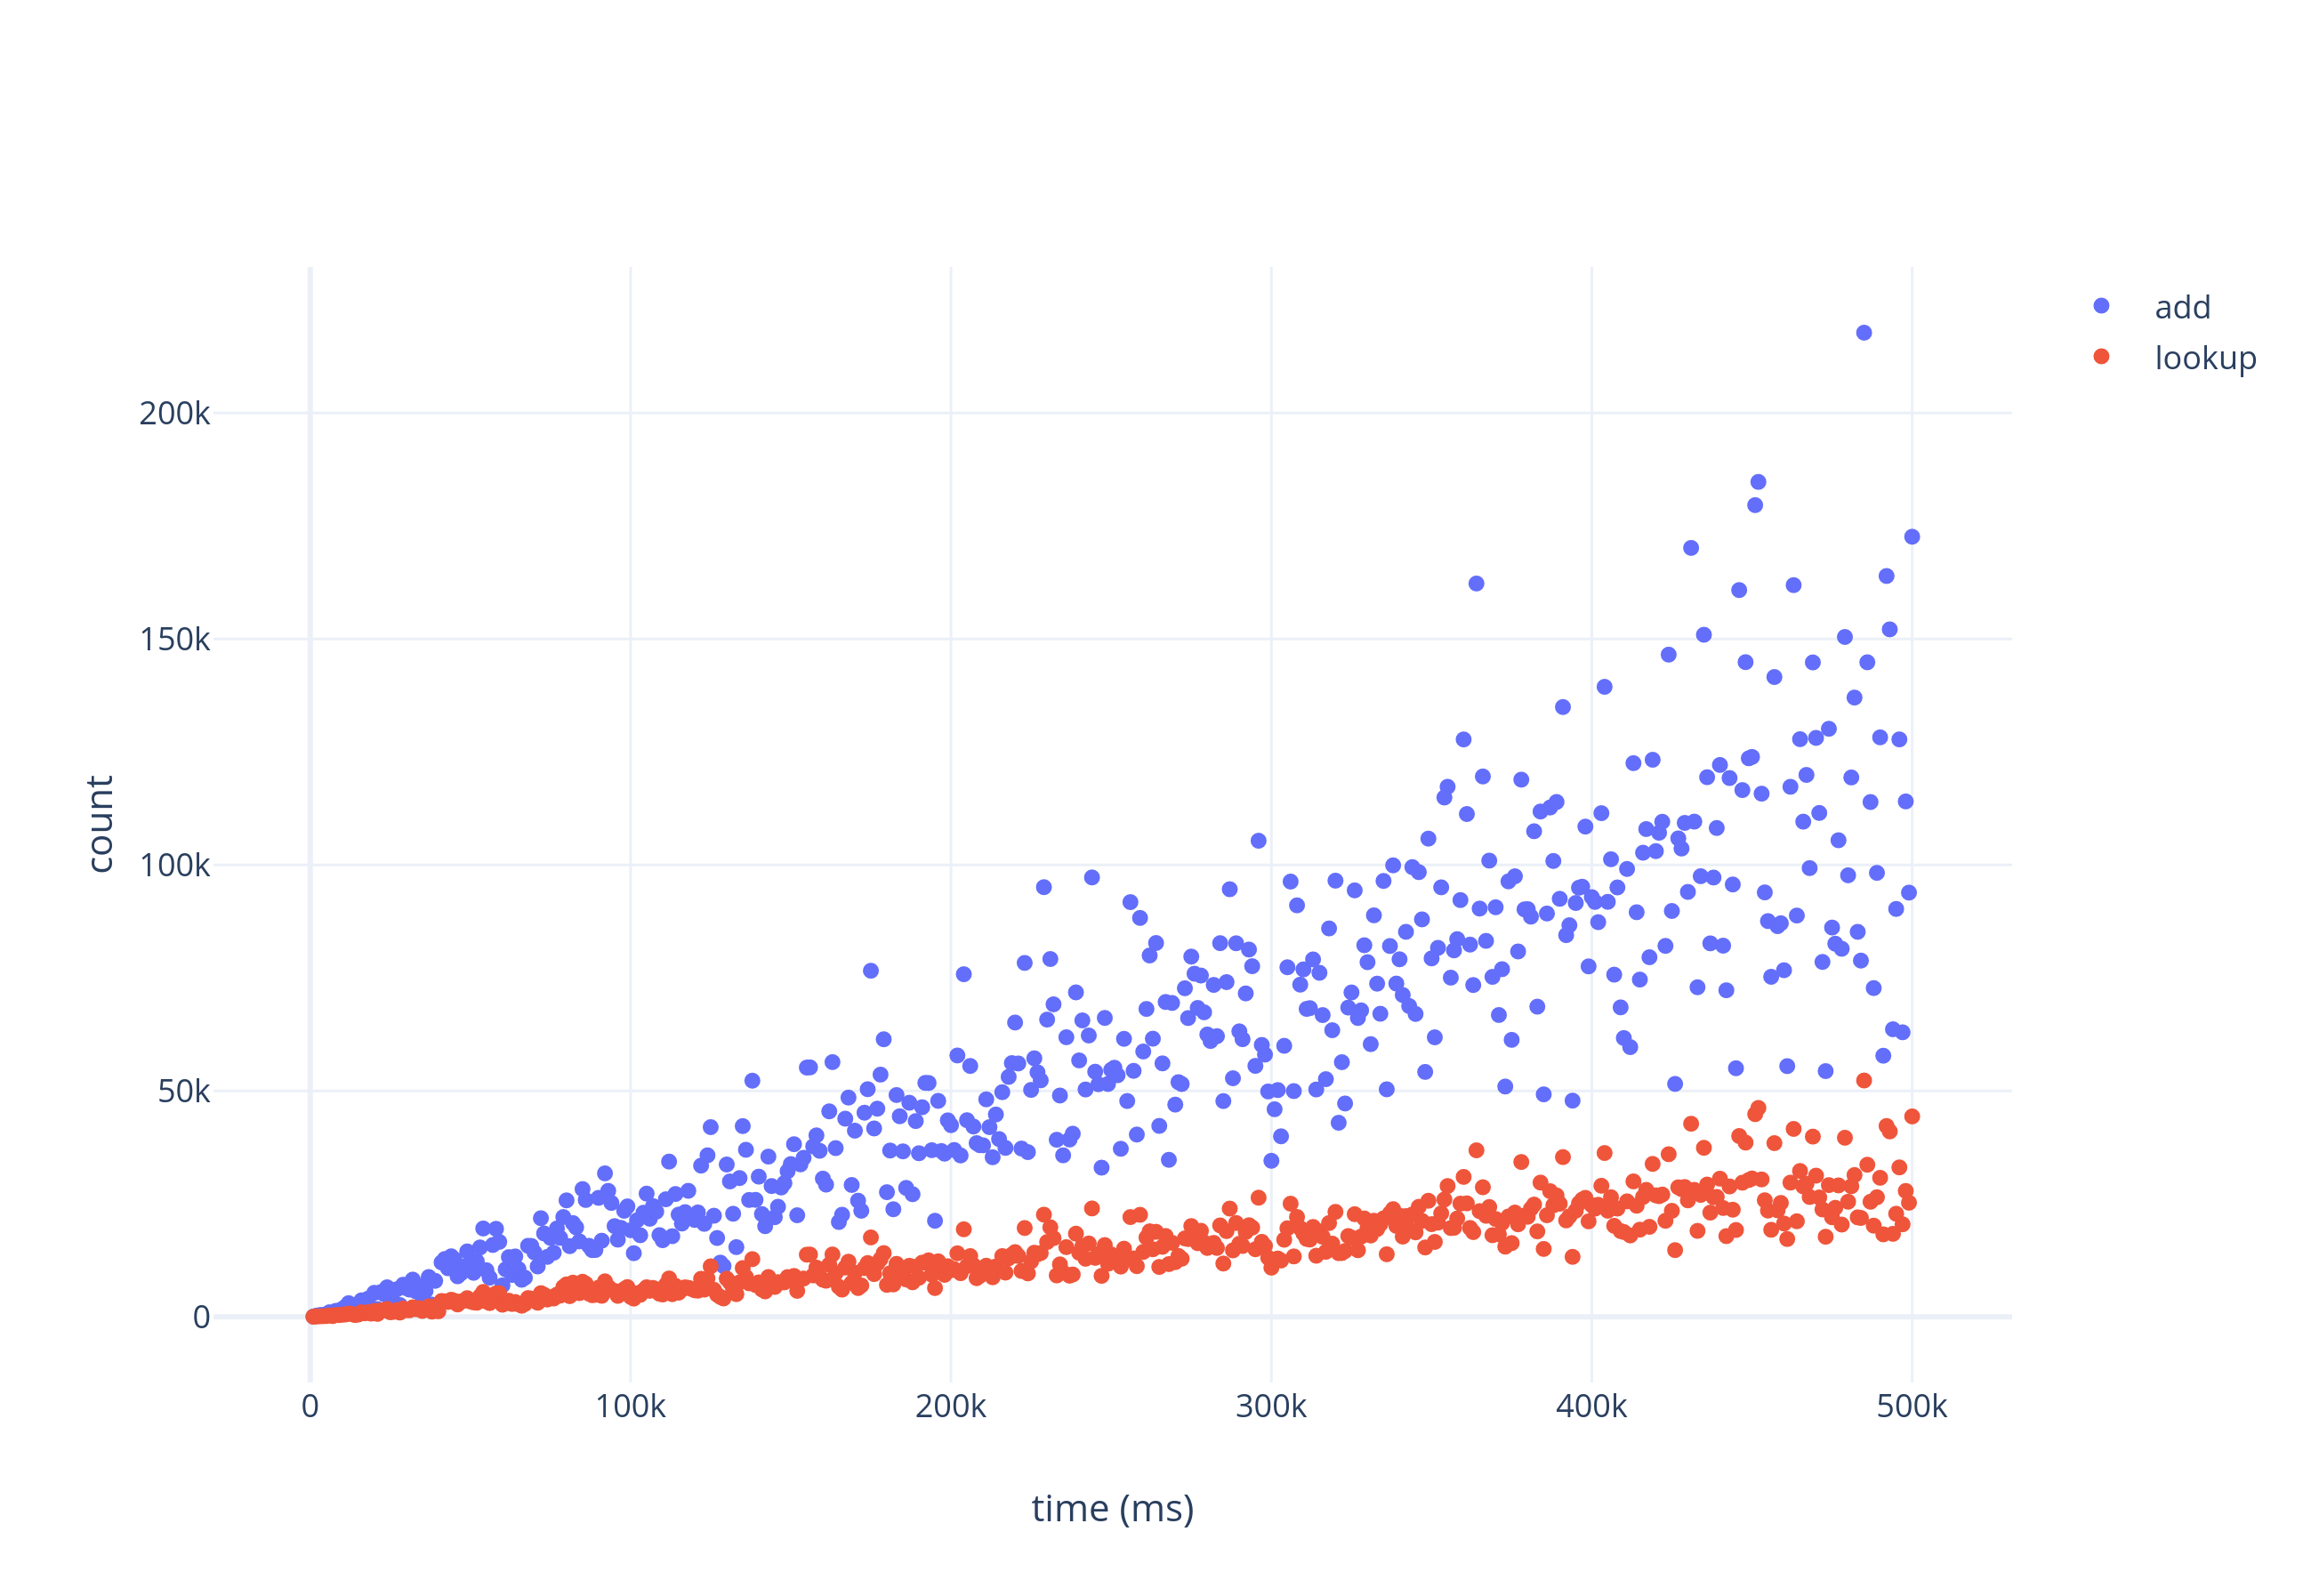
\includegraphics[width=\textwidth]{r_benchmark_non_empty_list}
    \caption{Some caption here}
\end{figure}


As can be seen, the graph looks to be ordo $O(n)$ which is different from a traditional $O(\log n)$ of a binary tree. Two explanations for this: a) the benchmark measures the total time taken for all elements to be added (instead of a single element in each iteration) and b) inefficiencies in Elixir pattern matching which may have influenced our results. 

\end{document}